%%%%%%%%%%%%%%%%%%%%%%%%%%%%%%%%%%%%%%%%%%%%%%%%%%%%%%%%%%%%%%%%%%%%
%% I, the copyright holder of this work, release this work into the
%% public domain. This applies worldwide. In some countries this may
%% not be legally possible; if so: I grant anyone the right to use
%% this work for any purpose, without any conditions, unless such
%% conditions are required by law.
%%%%%%%%%%%%%%%%%%%%%%%%%%%%%%%%%%%%%%%%%%%%%%%%%%%%%%%%%%%%%%%%%%%%

\documentclass[aspectratio=169]{beamer}
\usetheme[faculty=fi]{fibeamer}
\usepackage[utf8]{inputenc}
\usepackage[
  main=spanish, %% By using `czech` or `slovak` as the main locale
                %% instead of `english`, you can typeset the
                %% presentation in either Czech or Slovak,
                %% respectively.
  english,czech, slovak %% The additional keys allow foreign texts to be
]{babel}        %% typeset as follows:
%%
%%   \begin{otherlanguage}{czech}   ... \end{otherlanguage}
%%   \begin{otherlanguage}{slovak}  ... \end{otherlanguage}
%%
%% These macros specify information about the presentation
\title{Introducción a JS} %% that will be typeset on the
\subtitle{Taller parte 1 de 3} %% title page.
\author{
  Rodrigo Francisco \\
  Armando Rivera
}
%% These additional packages are used within the document:
\usepackage{ragged2e}  % `\justifying` text
\usepackage{booktabs}  % Tables
\usepackage{tabularx}
\usepackage{tikz}      % Diagrams
\usetikzlibrary{calc, shapes, backgrounds}
\usepackage{amsmath, amssymb}
\usepackage{url}       % `\url`s
\usepackage{listings}  % Code listings
\usepackage{multicol}
\usepackage{float}
\usepackage{wrapfig}
\usepackage{subcaption}
\graphicspath{ {../introduccionJS.assets/} }
\frenchspacing

\begin{document}
  \shorthandoff{-}
  \frame[c]{\maketitle}

  \AtBeginSection[]{% Print an outline at the beginning of sections
    \begin{frame}<beamer>
      %\frametitle{Contenido de la sección \thesection}
      \frametitle{Agenda}
        {\small \tableofcontents[currentsection]}
    \end{frame}}

  \begin{darkframes}
    \section{Introducción}
    \subsection{¿Qué es JavaScript?}
    \begin{frame}{JavaScript}
      \framesubtitle{\alert{JavaScript (JS) es un lenguaje de programación} multiplataforma}%
      \begin{center}
        
\includegraphics[width=8cm]{download}
      \end{center}
      \begin{itemize}
        \item Se considera un lenguaje orientado a objetos.
        \item Es un lenguaje basado en prototipos.
        \item Es un lenguaje interpretado (o just-in-time compiled).
      \end{itemize}
    \end{frame}


    \begin{frame}{JavaScript}
      \framesubtitle{\alert{JavaScript (JS) es un lenguaje de programación} multiplataforma}%
      \begin{itemize}
        \item Java y Javascript no tienen relación como lenguajes de programación.
        \item Las implementación de JS se rigen por el estándar ECMA-262.
        \item El nombre oficial del lenguaje es ECMAScript.
      \end{itemize}
    \end{frame}

    \begin{frame}[label=javascript]{JavaScript}
      \framesubtitle{\alert{JavaScript (JS) es un lenguaje de programación} multiplataforma}%
      \begin{itemize}
        \item Fue inventado en 1995 por Brendan Eich
        \item JS originalmente se creo para \textit{darle vida} a los navegadores.
        \item JS nació cómo un lenguaje del lado del cliente.
      \end{itemize}
    \end{frame}

    \subsection{¿Por qué aprender JS?}

    \begin{frame}{¿Por qué aprender JS?}
      \begin{center}
        
\includegraphics[width=0.7\textwidth]{jslearn}
      \end{center}
    \end{frame}

    \begin{frame}{¿Por qué aprender JS?}
      \framesubtitle{Existen muchas razones para aprender JS}

      \begin{columns}[T]
        \begin{column}{.5\textwidth}
    % Your text here
          \begin{itemize}
            \item Se pueden crear aplicaciones para casi todas las plataformas
            \item MongoDB y CouchDB usan javacript como su lenguaje de programación por defecto.
            \item Existen librerías/paquetes desarrolladas por la comunidad para casi todo tipo de requerimientos
          \end{itemize}
        \end{column}

        \begin{column}{.5\textwidth}
          % Your image included here
          \centering
        
\includegraphics[width=4cm]{mongo}
        \vspace{4mm}
        
\includegraphics[width=6cm]{download-1589848489734}
        \end{column}

      \end{columns}

    \end{frame}

    \begin{frame}{¿Por qué aprender JS?}
      \framesubtitle{Ventajas y desventajas}
      \textbf{Ventajas}
      \begin{itemize}
        \item Simplicidad. La sintaxis de javascript es muy sencilla.
        \item Populariad. Javascript es un lenguaje muy popular lo cual le garantiza tener soluciones implementadas por la comunidad para casi todas las necesidades.
        \item Interoperable. Javascript puede ser usado en junto con otros lenguajes de programación como Pearl y PHP.
        \item Funcionalidad extendida. Js permite extender la funcionalidad de algunos sitios web al incorporar scripts de js a estos.
        \item Rápido. Js tiende a ser un lenguaje rápido siempre que no tenga que obtener recursos externos.
      \end{itemize}
    \end{frame}

    \begin{frame}{¿Por qué aprender JS?}
      \framesubtitle{Ventajas y desventajas}
      \textbf{Desventajas}
      \begin{itemize}
        \item Vulnerabilidades del lado del cliente. Al ser un lenguaje del lado del cliente en ocasiones se suelen encontrar un bug que puede ser explotado para propósitos malicisos.

        \item Soporte de navegadores. En pleno 2020 esto ya no es una desventaja, actualmente todos los navegadores soportan JS en sus últimas versiones.

        \item Tricky language. A veces un puede tener dolores de cabeza al debugear un programa escrito en JS por que a veces hace varias asumpciones implicitas.
      \end{itemize}

    \end{frame}

    \subsection{Evolución del lenguaje}
    \begin{frame}{Evolución del lenguaje}
      \framesubtitle{ES5, ES6}
      En las primeras versión del lenguaje hasta la versión ES5, no se incorporaban clases ni exponenciación en la versión ES6.\\

      ES6 tiene las siguientes características:

      \begin{multicols}{2}
        \begin{itemize}
          \item JavaScript let
          \item JavaScript const
          \item JavaScript Arrow Functions
          \item JavaScript Classes
          \item Parámetros con valores por defecto
          \item Array.find()
          \item Array.findIndex()
          \item Exponentiation (**) (EcmaScript 2016)
        \end{itemize}
      \end{multicols}
    \end{frame}

    \subsection{Motores de JS}
    \begin{frame}{Motores de JS}
      \framesubtitle{Spider Monkey, V8, JScript}
      Google, Mozilla y Microsoft tiene sus propios motores de JS

      \begin{itemize}
          \item Spider Monkey es el nombre del motor de JS de Mozilla
          \item V8 es el motor de JS de Google Chrome
          \item Jscript es desarrollado por Microsoft.
      \end{itemize}
    \end{frame}

    \subsection{Herramientas para ejecutar JS}
    \begin{frame}{Herramientas para ejecutar JS}
      \framesubtitle{PlayCode,JSFiddle}

      \begin{itemize}
        \item JavaScript.com (\url{https://www.javascript.com/try})
        \item PlayCode (\url{https://playcode.io/})
        \item ES6 console (\url{https://es6console.com/})
        \item jsconsole (\url{https://jsconsole.com/})
        \item jsfiddle (\url{https://jsfiddle.net/})
        \item Plunker (\url{https://plnkr.co/})
        \item JSbin (\url{https://jsbin.com/?html,output})
        \item CodePen (\url{https://codepen.io/})
        \item Stackblitz (\url{https://stackblitz.com/})
      \end{itemize}
    \end{frame}
    \subsection{Typescript}
    \begin{frame}{Typescript}
      \framesubtitle{El hermano perdido de JS}
        TypeScript es un lenguaje de programación de código abierto desarrollado y
        mantenido por Microsoft.
        \begin{center}
          
\includegraphics[width=7cm]{download.jpeg}
        \end{center}

    \end{frame}
    \subsection{¿Dónde encontrar información?}
    \begin{frame}{Referencias}
      \framesubtitle{Docs, MDN}
      \begin{itemize}
        \item La mejor documentación que he tenido oportunidad de leer está en la página  de desarolladores de Mozilla.
        \begin{itemize}
          \item MDN web doc (\url{https://developer.mozilla.org/en-US/docs/Web/JavaScript})
          \item JavaScript reference (\url{https://developer.mozilla.org/en-US/docs/Web/JavaScript/Reference})
        \end{itemize}
        \item w3schools.com (\url{https://www.w3schools.com/Js/})
        \item javascript.info(\url{https://javascript.info/})
        \item What the f*ck is JavaScript? (\url{https://github.com/denysdovhan/wtfjs})
        \item jsher (\url{https://www.jshero.net/en/success.html})

      \end{itemize}

    \end{frame}

    \section{¡A programar!}
    \subsection{Sintaxis básica}
    \begin{frame}{Sintaxis básica}
      \framesubtitle{Las reglas}
      \begin{itemize}
        \item JS es case-sensitive, sensible a mayúsculas y minúsculas
        \item Usa el conjunto de caracteres Unicode
        \item El punto y coma (;) son es necesario para separar sentencias (instrucciones).
      \end{itemize}

      Un programa de computadora es una lista de \textit{instrucciones} para ser \textit{ejecutadas} por una computadora.\\

      En un lenguaje de programación, estas instrucciones de programación se denominan alert{sentencias}.\\

      Un programa de JavaScript es una lista de sentencias/instrucciones de programación.\\
    \end{frame}

    \begin{frame}{Sintaxis básica}
      \framesubtitle{Palabrar reservadas}
      \begin{center}
        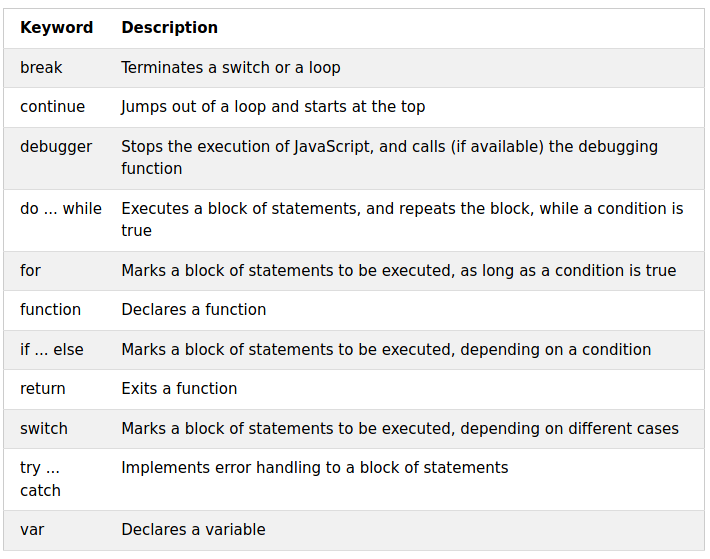
\includegraphics[width=.6\textwidth]{reservadas}
      \end{center}
    \end{frame}

    \begin{frame}{Sintaxis básica}
      \framesubtitle{Comentarios}
      Los comentarios son sentencias o comentarios (valga la redundancia) que no serán tomados en cuenta por el intérprete.\\

      Para poner comentarios en JS tenemos las siguientes opciones.
      \begin{itemize}
        \item Comentario de una línea, se utiliza \texttt{//}
        \item Comentario de multiples líneas: Tiene un inicio y un fin
        \begin{itemize}
          \item El inicio se denota con /* y el fin com */
        \end{itemize}
      \end{itemize}
    \end{frame}

    \subsection{Variables y tipos de datos}
    \begin{frame}{¿Qué es un variable?}
      \framesubtitle{Declaración de variables, var, const, let}

      \begin{columns}[T]
       \begin{column}{.5\textwidth}
    % Your text here
         Una variable es donde se guarda (y se recupera) datos que se utilizan en un programa.\\

         Para declarar una variable en JS se puede hacer de 3 formas
         \begin{itemize}
           \item Utilizando la palabra reservada var
           \item Utilizando la palabra reservada const
           \item Utilizando la palabra reservada let
         \end{itemize}
       \end{column}
       \begin{column}{.5\textwidth}
    % Your image included here
        \centering
       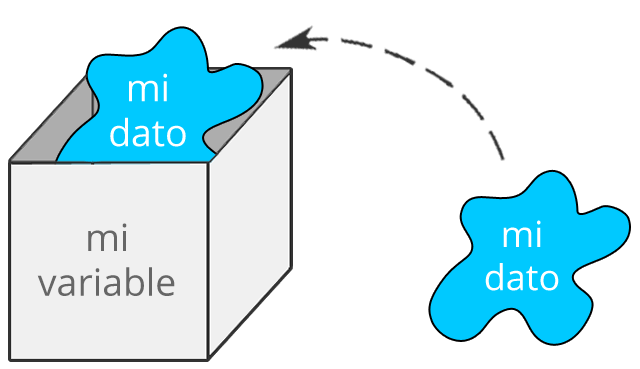
\includegraphics[width=7cm]{variable}
       \end{column}
     \end{columns}

    \end{frame}

    \begin{frame}{Variables}
      \framesubtitle{Indentificadores}
      Los identificadores se usan para nombrar variables (y palabras clave, funciones y etiquetas). \\

      Todas las variables de JavaScript deben identificarse con nombres únicos (identificadores).
    \end{frame}

    \begin{frame}{Variables}
      \framesubtitle{Reglas para los indentificadores}
      Las reglas generales para construir nombres para variables (identificadores únicos) son:
      \begin{itemize}
        \item Los nombres pueden contener letras, dígitos, guiones bajos y signos de dólar.
        \item Los nombres deben comenzar con una letra
        \item Los nombres también pueden comenzar con \$ y \_
        \item Los nombres distinguen entre mayúsculas y minúsculas (y e Y son variables diferentes)
        \item Las palabras reservadas (como las palabras clave de JavaScript) no se pueden usar como nombres
      \end{itemize}
    \end{frame}

    \begin{frame}{Tipos de datos}
      \framesubtitle{Según ECMAScript}
      En total tenemos 8 tipos de datos.
      \begin{itemize}
        \item Siete tipos de datos que son primitivos:
        \begin{itemize}
          \item Boolean. Verdadero y falso.
          \item null. Una palabra clave especial que denota un valor nulo.
          \item undefined. Una propiedad de nivel superior cuyo valor no está definido.
          \item Number. Un número entero o de coma flotante. Por ejemplo: 42 o 3.14159.
          \item BigInt. Un entero con precisión arbitraria. Por ejemplo: 9007199254740992n.
          \item String. Una secuencia de caracteres que representan un valor de texto. Por ejemplo: "Hola"
          \item Símbolo. (nuevo en ECMAScript 2015). Un tipo de datos cuyas instancias son únicas e inmutables.
        \end{itemize}

        \item y Object
      \end{itemize}

    \end{frame}

    \begin{frame}{Tipos de datos}
      \framesubtitle{Numbers}
      Los tipos Number y BigInt se pueden escribir en decimal (base 10), hexadecimal (base 16), octal (base 8) y binario (base 2).
      \begin{itemize}
        \item Un literal numérico decimal es una secuencia de dígitos sin un 0 inicial (cero).
        \item Un 0 inicial (cero) en un literal numérico, o un 0o inicial (ó 0O) indica que está en octal.
        \item Un 0x inicial (o 0X) indica un tipo numérico hexadecimal.
        \item Si al número se le agrega una n al final se convierte en un BigInt
        \item Un 0b inicial (o 0B) indica un literal numérico binario.
      \end{itemize}
    \end{frame}

    \begin{frame}{Tipos de datos}
      \framesubtitle{Strings}
      Caracteres especiales
      \begin{center}
        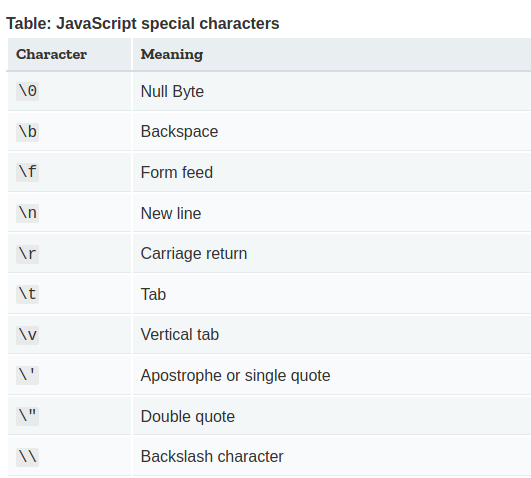
\includegraphics[width=.45\textwidth]{caracteres}
      \end{center}
    \end{frame}


    \subsection{Control de flujo y operadores}
    \begin{frame}{Operadores}
      \framesubtitle{Operadores de comparación}
      \begin{center}
        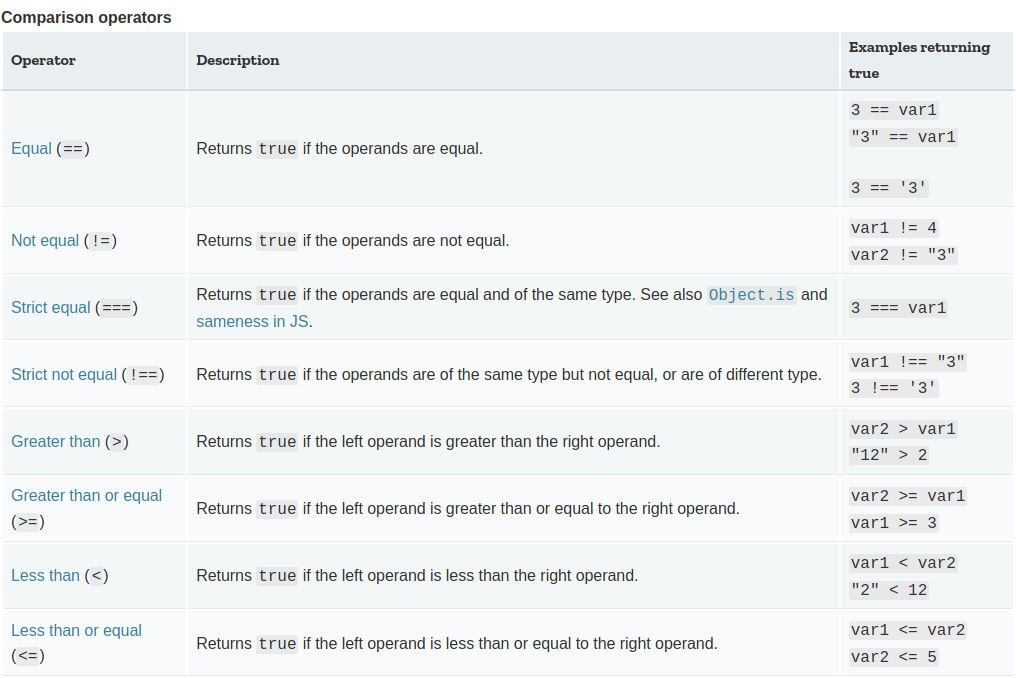
\includegraphics[width=.7\textwidth]{comparacion}
      \end{center}

    \end{frame}

    \begin{frame}{Operadores}
      \framesubtitle{Operadores aritméticos}
      \begin{center}
        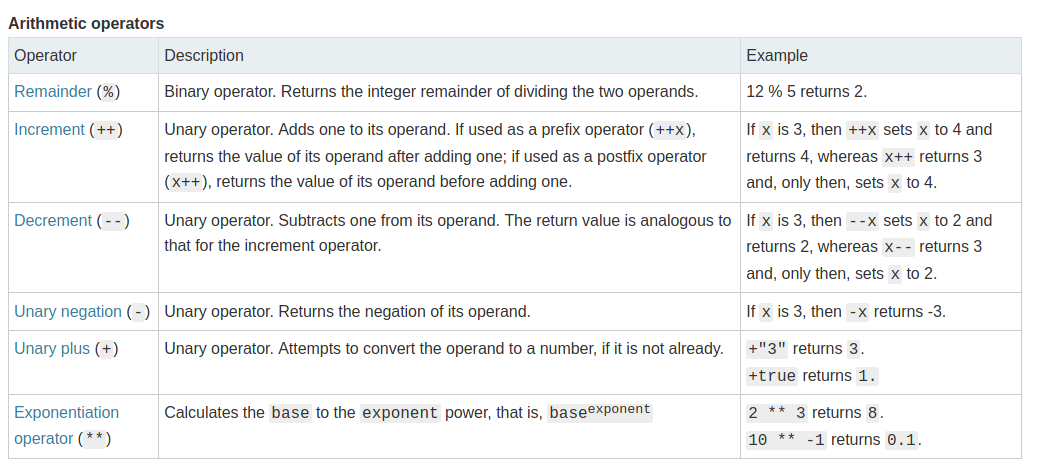
\includegraphics[width=.8\textwidth]{aritmeticos}
      \end{center}

    \end{frame}

    \begin{frame}{Operadores}
      \framesubtitle{Operadores bit a bit}
      \begin{center}
        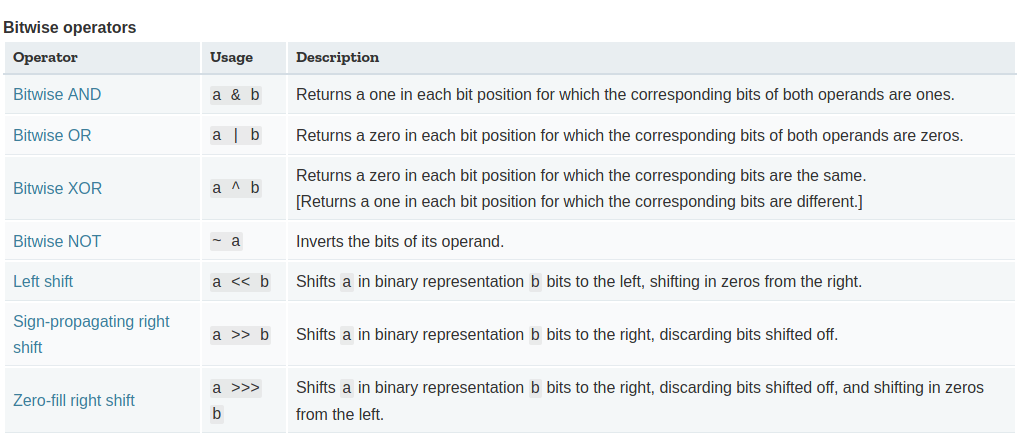
\includegraphics[width=.8\textwidth]{bitwise}
      \end{center}

    \end{frame}

    \begin{frame}{Operadores}
      \framesubtitle{Operadores lógicos}
      \begin{center}
        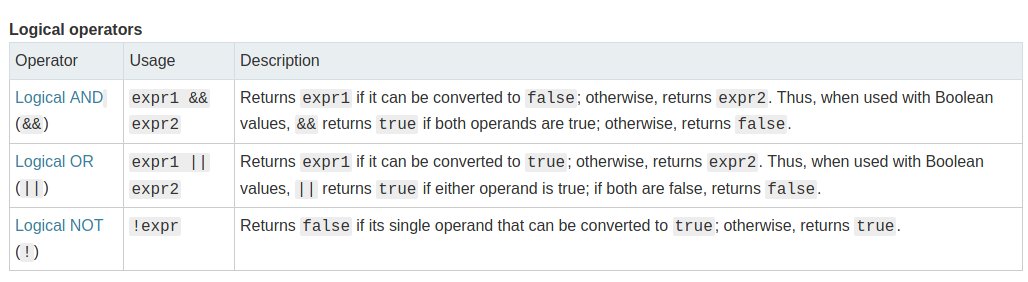
\includegraphics[width=.9\textwidth]{logical}
      \end{center}

    \end{frame}

    \defverbatim[colored]\sentif{
      \begin{lstlisting}[language=C,tabsize=2]
        if (condition_1) {
          statement_1;
        } else if (condition_2) {
          statement_2;
        } else if (condition_n) {
          statement_n;
        } else {
          statement_last;
        }
    \end{lstlisting}}

    \begin{frame}{Estructuras de control}
      \framesubtitle{if, else, else if}
      La instrucción if se usa para especificar un bloque de código Jque se ejecutará si una condición es verdadera.
      \begin{figure}[H]
        \begin{subfigure}{.7\textwidth}
          \begin{block}{Sentencia if}
            \sentif
          \end{block}
        \end{subfigure}
      \end{figure}
    \end{frame}

    \begin{frame}{Estructuras de control}
      \framesubtitle{Valores \alert{falsy}}
      Los siguientes valores se evalúan como falsos (también conocidos como valores Falsy):
      \begin{itemize}
        \item false
        \item undefined
        \item null
        \item 0
        \item NaN
        \item the empty string (``")
      \end{itemize}

    \end{frame}

    \defverbatim[colored]\ternary{
      \begin{lstlisting}[language=C,tabsize=2]
        condition ? val1 : val2

        var status = (age >= 18) ? 'adult' : 'minor';
    \end{lstlisting}}

    \begin{frame}{Estructuras de control}
      \framesubtitle{Operador ternario}
      Si la condición es verdadera, el operador tiene el valor que esta después del signo de interrogación. De lo contrario, tiene el valor que está después de los 2 puntos.

      \begin{figure}[H]
        \begin{subfigure}{.7\textwidth}
          \begin{block}{Operador ternario u Operador condicional}
            \ternary
          \end{block}
        \end{subfigure}
      \end{figure}

    \end{frame}

    \defverbatim[colored]\switch{
      \begin{lstlisting}[language=C,tabsize=2]
      switch (expression) {
        case label_1:
          statements_1
          [break;]
        case label_2:
          statements_2
          [break;]
          . . .
        default:
          statements_def
          [break;]
      }
    \end{lstlisting}}

    \begin{frame}{Estructuras de control}
      \framesubtitle{switch}

      \begin{columns}[T]
         \begin{column}{.5\textwidth}
            La instrucción \texttt{switch} permite que un programa evalúe una expresión e intente hacer coincidir el valor de la expresión con una etiqueta de caso. Si se encuentra una coincidencia, el programa ejecuta la declaración asociada.
         \end{column}
         \begin{column}{.5\textwidth}
         \begin{block}{Sentencia switch}
            \switch
         \end{block}
         \end{column}
       \end{columns}

    \end{frame}

    \defverbatim[colored]\for{
      \begin{lstlisting}[language=C,tabsize=2]
      for ([initialExpression]; [condition]; [incrementExpression])
        statement
    \end{lstlisting}}

    \begin{frame}{Estructuras de iteración}
      \framesubtitle{for}
      Un ciclo for se repite hasta que una condición especificada se evalúe como falsa.
      \begin{figure}[H]
        \begin{subfigure}{.9\textwidth}
          \begin{block}{Sentencia for}
            \for
          \end{block}
        \end{subfigure}
      \end{figure}
    \end{frame}

    \defverbatim[colored]\while{
      \begin{lstlisting}[language=C,tabsize=2]
      while (condition)
        statement
    \end{lstlisting}}

    \begin{frame}{Estructuras de iteración}
      \framesubtitle{while}
      Una sentencia while ejecuta sus sentencias siempre que una condición especificada se evalúe como verdadera.

      \begin{figure}[H]
        \begin{subfigure}{.7\textwidth}
          \begin{block}{Sentencia while}
            \while
          \end{block}
        \end{subfigure}
      \end{figure}

    \end{frame}

    \defverbatim[colored]\dowhile{
      \begin{lstlisting}[language=C,tabsize=2]
      do
        statement
      while (condition);
    \end{lstlisting}}

    \begin{frame}{Estructuras de iteración}
      \framesubtitle{do while}
      La instrucción do ... while se repite hasta que una condición específica se evalúa como falsa.

      \begin{figure}[H]
        \begin{subfigure}{.7\textwidth}
          \begin{block}{Sentencia do while}
            \dowhile
          \end{block}
        \end{subfigure}
      \end{figure}
    \end{frame}

    \subsection{Arreglos}
    \begin{frame}{Arreglos}
      \framesubtitle{Las características importantes son ...}

      \alert{Un arreglo es una variable especial, que puede contener más de un valor a la vez.}\\

      Un arreglo puede contener muchos valores con un solo nombre, y puede acceder a los valores haciendo referencia a un número de índice.\\

      Los arreglos son un tipo especial de objetos. \\

    \end{frame}
    \subsection{Funciones}
    \begin{frame}{Funciones}
      \framesubtitle{Definición}
      Una función de JavaScript es un bloque de código diseñado para realizar una tarea en particular.\\

      Una definición de función (también llamada declaración de función o declaración de función) consiste en la palabra clave de función, seguida de:
      \begin{itemize}
        \item El nombre de la función.
        \item Una lista de parámetros para la función, entre paréntesis y separados por comas.
        \item Las declaraciones de JavaScript que definen la función, encerradas entre llaves, \{...\}
      \end{itemize}
    \end{frame}

    \begin{frame}{Funciones}
      \framesubtitle{Tipos de funciones}
      \begin{itemize}
        \item Funciones anónimas
        \item Funciones anidadas
        \item Funciones con parametro por defecto
        \item Funciones que reciben funciones
        \item Paso por valor y paso por referencia
        \item Arrow Function (introducción)
      \end{itemize}
    \end{frame}

    \section*{Referencias y Bibliografía}
    \begin{frame}[label=bibliography]{Referencias y Bibliografía}
      \framesubtitle{MDN,w3schools}
      \begin{thebibliography}{9}
        \bibitem{mdn}
            Mozilla Developer Network.
            \emph{JavaScript}.
            Disponible en \url{https://developer.mozilla.org/en-US/docs/Web/javascript}
        \bibitem{w3schools}
            w3schools.
            \emph{JavaScript Tutorial}.
            Disponible en \url{https://www.w3schools.com/Js/}
        \bibitem{freecodecamp}
            Free Code Camp,
            \emph{The Best JavaScript Examples}.
            Disponible en \url{https://www.freecodecamp.org/news/javascript-example/}

        \bibitem{thefuckisjs}
            Denys Dovhan.
            \emph{What the f*ck JavaScript?}.
            Disponible en \url{https://github.com/denysdovhan/wtfjs}
      \end{thebibliography}
    \end{frame}

    \begin{frame}{Material y ejemplos}
      \framesubtitle{Link de github}
      \begin{center}
        {\Large
          \url{https://github.com/rhofp-cursos/curso_js}
        }
      \end{center}
    \end{frame}

  \end{darkframes}

\end{document}
